\chapter{Instrumentierung}

\section{Trace}\label{Chap:Instrumenter-Sec:Trace}
Wie bereits in dem vorherigen Kapitel beschrieben soll, um das 
Programm analysieren zu können ein Trace aufgezeichnet werden.\\
Anders als in vielen anderen Programmen, welche den Trace von Go-Programmen
analysieren, wie z.B.~\cite{GoAt2} oder~\cite{GoVis} wird dabei der Tracer 
selbst implementiert und basiert nicht auf dem Go-Runtime-Tracer~\cite{GoRunTrace}. 
Dies ermöglicht es, den Tracer genau auf die benötigten Informationen zuzuschneiden
und so einen geringeren negativen Einfluss auf die Laufzeit des Programms zu erreichen.\\\\
Um diesen Trace zu erzeugen, werden die Standartoperation auf Go durch Elemente
des Tracers ersetzt. Die Funktionsweisen dieser Ersetzungen sind im folgenden 
angegeben. Dabei werden nur solche Ersetzungen angegeben, welche direkt 
für die Erzeugung
des Traces notwendig sind. Zusätzlich werden noch 
weitere Ersetzungen durchgeführt, wie z.B. die Ersetzung der Erzeugung von 
Mutexen und Channel von den Standardvarianten zu den Varianten des Tracers.
Hierbei wird auch die Größe jedes Channels gespeichert.
Dies werden in der Übersicht zur Vereinfachung nicht betrachte. Auch werden 
in der Übersicht nur die Elemente betrachtet, die für die Durchführung der 
Operation und dem Aufbau des Traces benötigt werden. Hilfselemente, wie z.B. 
Mutexe, welche verhindern, dass mehrere Routinen gleichzeitig auf die selbe 
Datenstruktur, 
z.B. die Liste der Listen, welche die Traces für die einzelnen Routinen 
speichern, zugreifen, werden nicht mit angegeben. Dabei sei $c$ ein 
Zähler, $nR$ ein Zähler für die Anzahl der Routinen, $nM$ ein Zähler für die 
Anzahl der Mutexe und $nC$ ein Zähler für die Anzahl der Channels. $nM$ und $nC$
werden bei der Erzeugung eines neuen Mutex bzw. eines neuen Channels atomarisch 
Inkrementiert. Den erzeugten Elementen wird er neue Wert als $id$ zugeordnet. All diese 
Zähler seien global und zu Beginn als $0$ initialisiert. Außerdem bezeichnet 
$mu$ einen Mutex, $rmu$ einen RW-Mutex, $ch$ einen Channel und $B$ bzw. $B_i$
mit $i\in\mathbb{N}$ den 
Körper einer Operation. Zusätzlich
sei $id$ die $Id$ der Routine, in der eine Operation ausgeführt wird,
$[signal(t, i)]^{id}$ bedeute, dass der das entsprechende Element (hier als 
Beispiel $signal(t, i))$, in den Trace der Routine mit id $id$ eingeführt wird
und $[+]^i$ bedeute, das in die Liste der Traces ein neuer, leerer Trace 
eingefügt wird, welcher für die Speicherung des Traces der Routine $i$ 
verwendet wird. 
$\langle a|b\rangle$ bedeutet, dass ein Wert je nach Situation auf $a$ oder $b$ gesetzt 
wird. Welcher Wert dabei verwendet wird, ist aus der obigen Beschreibung der 
Trace-Elemente erkennbar. $\text{e}_1$ bis $\text{e}_n$ bezeichnet die Selektoren in einem Select statement.
$\text{e}_i^*$ bezeichnet dabei einen Identifier für einen Selektor, der sowohl die 
Id des beteiligten Channels beinhaltet, als auch die Information, ob es sich um ein 
Send oder Receive handelt und $\text{e}_i^m$ die Message, die in einem Case 
empfangen wurde. 
\begin{tabular}{lcl}
  go B & $\Rightarrow$ & nr := atomicInc(nR); ts := atomicInc(c); [ signal(ts, nr) ]$^\text{nr}$;\\
    & & [+]$^\text{nr}$; go \{ ts' := atomicInc(c); [ wait(ts, nr) ]$^\text{id}$; B\};\\
  ch <- i & $\Rightarrow$ & ts := atomicInc(c); [ pre(ts, ch.id, true) ]$^\text{id}$; ch <- \{i, id, ts\};\\
    & & ts' := atomicInc(c); [ post(ts', ch.id, true, id) ]$^\text{id}$\\
  <- ch & $\Rightarrow$ & ts := atomicInc(c); [ pre(ts, ch.id, false) ]$^\text{id}$;\\
    & & \{i, id\_send, ts\_send\} := <-c; ts' := atomicInc(c);\\
    & & [ post(ts', ch.id, false, id\_send, ts\_send) ]$^\text{id}$; return i;\\
  close(ch) & $\Rightarrow$ & ts := atomicInc(c); close(ch); [ close(ts, ch.id) ]$^\text{id}$\\
  select(e$_\text{i} \leadsto \text{B}_\text{i}$) & $\Rightarrow$ & ts := atomicInc(c); [ pre(ts, e$_1^*$, $\ldots$, e$_n^*$, false) ]$^\text{id}$;\\
    & & select(e$_\text{i} \leadsto$ \{ ts' := atomicInc(c);\\
    & & [ $\langle \text{post(ts, e$_\text{i}$.ch, false, e$_\text{i}^\text{m}$.id\_send, e$_\text{i}^\text{m}$.ts\_send)}\ |$ \\
    & & post(ts, e$_\text{i}$.ch, true, id) $\rangle$ ]$^\text{id}$ B$_\text{i}$\}) \\
  select(e$_\text{i} \leadsto \text{B}_\text{i}$ | B$_\text{def}$) & $\Rightarrow$ & ts := atomicInc(c); [ pre(ts, e$_1^*$, $\ldots$, e$_n^*$, false) ]$^\text{id}$;\\
    & & select(e$_\text{i} \leadsto$ \{ ts' := atomicInc(c);\\
    & & [ $\langle \text{post(ts, e$_\text{i}$.ch, false, e$_\text{i}^\text{m}$.id\_send, e$_\text{i}^\text{m}$.ts\_send)}\ |$ \\
    & & post(ts, e$_\text{i}$.ch, true, id) $\rangle$ ]$^\text{id}$ B$_\text{i}$\} |\\
    & & ts' := atomicInc(c); [ default(ts) ]$^\text{id}$; B$_\text{def}$) \\
  mu.(Try)Lock() & $\Rightarrow$ & ts := atomicInc(c);
    [ lock(ts, mu.id, $\langle \text{-|t}\rangle$, $\langle \text{0|1}\rangle$) ]$^\text{id}$;\\
    & & mu.(Try)Lock();\\
  mu.Unlock() & $\Rightarrow$ & ts := atomicInc(c); mu.Unlock(); [ unlock(ts, mu.id) ]$^\text{id}$;\\
  rmu.(Try)(R)Lock() & $\Rightarrow$ & ts := atomicInc(c); rmu.(Try)(R)Lock();\\
    & & [ lock(ts, rmu.id, $\langle \text{-|t|r|tr}\rangle$, $\langle \text{0|1}\rangle$) ]$^\text{id}$;\\
  rmu.Unlock() & $\Rightarrow$ & ts := atomicInc(c); rmu.Unlock(); [ unlock(ts, rmu.id) ]$^\text{id}$;
\end{tabular}
Für Receive, Send und Close auf Channels,  allen Operation auf Mutexen sowie 
der Erzeugung von Strukturen als Ersatz für die eigentlichen Mutexe und Channels 
sind Funktionen implementiert, welche die Entsprechenden Operationen 
ersetzen und dabei sowohl die Aufzeichnung in dem Trace, als auch die eigentlichen
Operationen durchführen. Hierbei sind besonders die Send- und Receive Operationen 
zu betrachten. Für den Trace muss dem Receive-Statement die Sender-Routine, sowie 
dessen momentane 
Zeitstempel bekannt sein. Daher wird bei der eigentlichen
Send-Operation nicht nur die eigentliche Information gesendet, sondern ein  
Objekt, welches die Information, sowie die Id der sendenden Routine und deren
Zeitstempel beinhaltet.\\Für die anderen Operationen sind Funktionen 
definiert, die in die entsprechenden Strukturen eingefügt werden, um so
die Aufzeichnung in dem Trace zu gewehrleisten. Die eigentlichen Operationen
werden in diesen Fällen aber weiterhin in dem eigentlichen Code vorgenommen.

\section{Select}\label{Chap:Inst-Sec:Select}
Neben den Ersetzungen der einzelnen Operationen, werden auch die Select-Statements 
verändert, um einen der Fälle bevorzugt auswählen zu können, wie in Kap.~\ref{Chap:Back-Sec:Select}.
beschrieben. Die Implementierung basiert dabei zum größten Teil auf~\cite{gfuzz}.
Abb.~\ref{Chap:Analyze-Sec:Channel-SubSec:Select-Fig:GFuzz_Inst} zeigt ein 
Beispiel für die Instrumentierung eines 
\begin{figure}[h!]
  \begin{minipage}[t]{0.3\textwidth}
    \lstinputlisting[xrightmargin=-50pt]{code/gfuzz-select-pre.txt}
  \end{minipage}
  \begin{minipage}[t]{0.65\textwidth}
    \lstinputlisting[xrightmargin=40pt]{code/gfuzz-select-post.txt}
  \end{minipage}
  \caption{Beispiel für die Order-Enforcement-Instrumentierung eines Select-Statements 
  vor (links) und nach der Implementierung (rechts). Ersetze $......$
  in dem Programm nach der Instrumentierung (rechts) durch das Programm vor der 
  Instrumentierung (links).~\cite[gekürzt]{gfuzz}}
  \label{Chap:Analyze-Sec:Channel-SubSec:Select-Fig:GFuzz_Inst}
\end{figure}
Die Select-Operation wird durch eine Switch-Operation auf der \texttt{Fetch-Order}
ersetzt. Die Fetch-Order speichert für jede Select-Operation den Index des bevorzugten
Case. Für eine gewisse, festgelegte Zeit $T$ wird somit nur auf die in der 
\texttt{Fetch-Order} spezifizierten Operation gewartet. Wird diese in der 
vorgegebenen Zeit nicht ausgeführt, geht das Programm wieder in die Ausführung
der ursprünglichen Select-Operation um zu verhindern, dass es zu einem 
Deadlock kommt, welcher in dem originalen-Code nicht vorgekommen wäre.
Das selbe gilt auch, wenn für die Select-Operation fälschlicherweise kein 
gültiges Case ausgewählt worden ist. Anders als in~\cite{gfuzz} beschrieben,
wird für ein Select in dem selben Durchlauf immer der selbe Channel priorisiert, 
auch wenn die Operation mehrfach durchlaufen wird. Um für jede Ausführung einen
eigenen Case zu priorisiere, müsste, da die Ordnung bereits vor dem 
Durchlauf festgelegt werden soll, der Ablauf des Programms bereits 
bekannt sein. Dies ist allerdings nur möglich, wenn die Wahl der Cases der 
Select-Operationen keine Einfluss auf die Ausführung anderer Select-Cases 
hat. Dass dadurch nicht alle möglichen Abläufe durchlaufen werden können, 
muss dabei in kauf genommen werden.







\section{Automatisierter Instrumenter}\label{Chap:Instrumenter-Sec:Instrumenter}
Um den Trace zu erzeugen, müssen verschiedene Operationen durch Funktionen
des Tracers ersetzt bzw. erweitert werden. Bei einem größeren 
Programmcode ist eine händische Instrumentierung nicht machbar.
Da sich der Tracer auch negativ auf die Laufzeit des Programms 
auswirken kann, ist es in vielen Situationen nicht erwünscht, ihn in den 
eigentlichen Release-Code einzubauen, sondern eher in eine eigenständige 
Implementierung, welche nur für den Tracer verwendet werden. Um dies zu
automatisieren wurde ein zusätzliches Programm implementiert, welches in der 
Lage ist, den Tracer in normalen Go-Code einzufügen.\\\\

Der automatische Instrumenter besteht aus zwei Teilen. 
Zum einen werden alle 
in dem Programm vorhandenen ``.go'' Dateien instrumentiert. 
Zum anderen 
wird, basierend auf einem Template, eine neue Main-Datei erzeugt.
Diese bestimmt die zu durchlaufenden Ordnungen der Select-Operationen 
und führt diese nacheinander aus. 

\subsection{Instrumentierung der Dateien}
Bevor die einzelnen Dateien instrumentiert werden, wird der Ordner mit 
dem originalen Code durchlaufen, und seine Ordnerstruktur in den 
Output-Ordner kopiert. Anschließend werden alle Dateien durchlaufen.
Handelt es sich nicht um ``.go'' Dateien werden sie einfach an die entsprechende 
Stelle im Output-Ordner kopiert. Handelt es sich um ``.go'' Dateien, dann wird 
der Programmcode so verändert, dass der erzeugte Code alle für den Analyzer 
notwendig Elemente enthält. Go besitzt in seiner Standart-Bibliothek ein 
Library zur Erzeugung und Bearbeitung des Abstract-Syntax-Trees einer 
Datei~\cite{ast-spec}. Zur Instrumentierung einer Datei wird dieser Baum 
mehrfach durchlaufen, dabei entsprechend angepasst und anschließend der 
veränderte AST als Code in der neuen Datei abgespeichert. Das mehrfache Durchlaufen 
ist notwendig, um Überschneidungen zwischen den einzelnen Teilen zu verhindern.
Der Baum wird insgesamt drei mal durchlaufen.
\paragraph{1. Durchlauf:} Im ersten Durchlauf wird der Import der 
GoChan-Bibliothek eingefügt und die Main-Funktion des 
Programms sowie Channels in Funktionsdeklarationen instrumentiert.
Zuerst wird in jede Datei der Import der GoChan-Bibliothek eingeführt. In Go 
müssen alle importierten Bibliotheken verwendet werden. Andernfalls kommt es 
zu einem Compiling-Error. Um zu verhindern, dass dies bei einer Datei, die weder
Mutex noch Channel-Operationen besitzt geschieht, wird nach der abgeschlossenen 
Instrumentierung das ``goimport'' tool aufgerufen, welches nicht verwendete import 
automatisch entfernt. Die Instrumentierung der Main-Funktion findet nur 
in der Main-Datei des Programms statt. Dabei wird der goChan-Analyzer initialisiert,
sowie den Start der Analyze durch eine defer-Statement vorbereitet. In der 
Initialisierung des Analyzers werden die Datenstrukturen zur Speicherung 
des Traces erzeugt. Außerdem wird eine zusätzliche Routine mit einem 
Timer gestartet. Läuft dieser Timer ab (default: 10s), nimmt der Analyzer an, 
dass es zu einem tatsächlichen Deadlock gekommen ist, und startet die Analyze, 
auch wenn das Programm noch nicht abgeschlossen ist. In diesem Fall wird das 
Programm nach der Analyze automatisch abgebrochen. Für Programme, die von 
selbst eine längere Laufzeit haben muss die Dauer des Timers entsprechen 
angepasst werden. Zusätzlich wird in die Datei mit der Main-Funktion eine 
globale Variable aufgenommen, welche die FetchOrder für die Select-Case 
des momentanen Durchlaufs speichert. Anschließend werden in allen Funktionen, 
welche Channels als Parameter oder Rückgabewerte haben, diese durch die 
entsprechenden Go-Chan-Objekte ersetzt.
\paragraph{2. Durchlauf} Im zweiten Durchlauf werden die restlichen 
Channel Operationen instrumentiert. Hierbei werden alle Knoten des 
AST durchlaufen. Beinhaltet dieser eine Channel-Operation (z.B. Erzeugung 
einses Channels, Send, Receive usw.) wird sie durch die entsprechende 
Operation aus dem Go-Chan Analyzer ersetzt. Dabei muss beachtet werden,
dass solche Operationen in den verschiedensten Operationen (z.B. in defer, 
range usw.) enthalten sein können, welche jeweils einzeln betrachtet und 
ersetzt werden müssen. Der Channel selber wird dabei durch ein Objekt ersetzt, 
welches den eigentlichen Channel, die Id des Channels, seine Kapazität sowie 
die Anzahl der bereits erfolgreich durchgeführten Send und Receive Operationen
speichert. Die Definition dieses Struct wird, wie die Funktionen auf diesem 
Objekt durch GoChan definiert.\\\\Auch die Erzeugung von neuen Go-Routinen 
wird hier instrumentiert. Ein Beispiel zur Instrumentierung der Erzeugung einer 
neuen Go-Routine findet sich in Abb.~\ref{Chap:Instrumenter-Sec:Instrumenter-Fig:GoRoutine}.
\begin{figure}[h!]
  \begin{minipage}[t]{0.3\textwidth}
    \lstinputlisting[xrightmargin=-5pt]{code/go_routine_pre.txt}
  \end{minipage}
  \begin{minipage}[t]{0.65\textwidth}
    \lstinputlisting[xrightmargin=-5pt]{code/go_routine_post.txt}
  \end{minipage}
  \caption{Instrumentierung der Erzeugung einer neuen Go-Routine. Links: vor der 
    Instrumentierung, rechts: nach der Instrumentierung.}
  \label{Chap:Instrumenter-Sec:Instrumenter-Fig:GoRoutine}
\end{figure}
\texttt{SpawnPre} erzeugt dabei das \texttt{signal} Element in dem Trace 
und gibt außerdem die Id der erzeugenden Routine zurück, welche in \texttt{SpawnPost}
für die Erzeugung des \texttt{wait} Elements benötigt wird. Das umschließen 
des ganzen mit einer weiteren Funktion erleichtert die Implementierung 
des Instrumenters, ist aber nicht unbedingt notwendig.\\\\
Zusätzlich werden auch die Select-Statements instrumentiert. 
Zum einen wird hier das Select-Statement wie in~\ref{Chap:Back-Sec:Select} 
beschrieben durch ein Switch-Statement mit mehreren Select-Statements 
ersetzt, um einen der Cases zu bevorzugen. 
Die Instrumentierung der Select-Statements für den Trace stellte dabei 
eine Komplikation da, da die Cases eines Select-Statements nur tatsächliche
Channel-Operationen akzeptiert, diese also nicht direkt durch die Ersatzfunktionen 
des Analyzers ersetzt werden können. Die Lösung besteht darin, die 
Erzeugung der Events für den Tracer von dem eigentlichen Select-Case Statement 
zu trennen. Ein Beispiel dazu findet sich in 
Abb.~\ref{Chap:Instrumenter-Sec:Instrumenter-Fig:SelectFull}.
\begin{figure}[h!]
  \begin{minipage}[t]{0.3\textwidth}
    \lstinputlisting[xrightmargin=-45pt]{code/select_full_pre.txt}
  \end{minipage}
  \begin{minipage}[t]{0.65\textwidth}
    \lstinputlisting[xrightmargin=-5pt]{code/select_full_post.txt}
  \end{minipage}
  \caption{Instrumentierung eines Select-Statements. Links: vor der 
    Instrumentierung, rechts: nach der Instrumentierung.}
  \label{Chap:Instrumenter-Sec:Instrumenter-Fig:SelectFull}
\end{figure}
Zuerst wird die \texttt{goChan.PreSelect} Funktion aufgerufen, welche das 
Pre-Event in dem Trace erzeugt. Die Parameter dieser Funktion geben an, 
ob das Select-Statement einen Default-Case besitzt (in diesem Fall false),
sowie für welche Channels es Cases gibt, und ob es sich bei diesen 
um Send- oder Receive-Statements handelt. Anders als in dem Original-Code 
werden in dem instrumentierten Code auf Channels nicht nur die Nachrichten selbst, 
sondern auch Informationen über die sendende Routine verschickt. Da in einem 
Select-Case die Channel-Operationen nicht direkt ersetzt werden können, 
müssen nun für alle Cases, welche durch eine Send-Operation ausgelöst werden 
diese Nachrichten erzeugt werden. In dem Beispiel git es einen Case, 
auf den dies Zutrifft. Durch \texttt{sel\_RAjWwhTH := goChan.BuildMessage(1)}
wird diese erzeugt. \texttt{RAjWwhTH} ist dabei lediglich eine zufällige 
Zeichenkette, um unterschiedliche Nachrichten voneinander trennen zu können. 
Anschließend beginnt das switch Statement. \texttt{goChanFetchOrder} ist 
dabei die globale Map, die für jedes Select-Statement den für diesen 
Durchlauf bevorzugte Case angibt. \texttt{1} ist dabei die Id des 
select-Cases. Dadurch, dass die Anzahl 
der möglichen Ids sehr groß gewählt ist und diese dann zufällig zugeteilt 
werden, ist die Wahrscheinlichkeit verschwindend gering, dass mehrere 
Select-Cases die selbe Id- erhalten.\\Auf den Cases werden nun normale 
Channel-Operationen ausgeführt. Da aber nicht nur die eigentlichen 
Nachrichten versendet werden, müssen bei Receive-Statements mit anschließendem 
Assignement die eigentliche Nachricht aus dem Channel extrahiert werden. Außerdem 
wird bei einem Send-Statement die Nachricht durch die vorher erzeugte ausgetauscht.
Innerhalb des Cases wird die \texttt{goChan.Post} Funktion aufgerufen, um wenn 
der Case ausgewählt wurde das \text{post}-Event in dem Trace zu erzeugen.\\
Neben der eigentlichen Instrumentierung der Select-Statements werden die Select-
Cases mit ihren Ids außerdem aufgezeichnet. Beinhaltet das Programm mindestens 
ein Select-Statement, so wird, nachdem der Baum vollständig durchlaufen wurde 
die Main-Funktion so verändert, dass es ein Command-Line-Argument \texttt{-order}
annehmen kann. Dieses beinhaltet einen String, in dem die \texttt{FetchOrder} für
den Programmdurchlauf an des Programm übergeben werden kann.
\paragraph{3. Durchlauf} Im dritten Durchlauf werden nun noch die Mutex-Operationen 
durch, von dem GoChan-Analyzer zur Verfügung gestellt Funktionen ersetzt, 
welche das eigentliche Locking als auch die Aufzeichnung des Traces übernehmen. 
Da es hierbei keine speziellen Strukturen wie select o.ä.\ gibt, ist eine 
einfache direkte Ersetzung der Operationen möglich. Die Objekte, welche die 
Mutexe dabei ersetzen speichern dabei lediglich den eigentlichen Mutex, welcher 
das Locking tatsächlich ausführt, sowie die Id des Mutex. Für Mutex und RW-Mutex 
ist dabei jeweils ein eigenes Objekt definiert.


\subsection{Neue Main-Datei}
Der in~\ref{Chap:Instrumenter-Sec:Instrumenter} erzeugt Code ist nun 
prinzipiell Lauffähig. Allerdings wird er nur einmal durchlaufen. Aufgrund der 
Select-Statements soll das Programm nun aber mehrfach, mit verschiedenen 
Select-Orders durchlaufen werden. Dazu wird eine neue Main-Datei erzeugt, mit 
welcher das eigentliche Programm gestartet wird. Diese Datei wird über ein 
Template erzeugt, mit welchem, basierend auf den Aufzeichnungen der instrumentierten 
Select-Cases die neue Datei erzeugt wird. Zuerst erzeugen wir eine Map, die 
für jedes Select-Statement die Anzahl der Cases, also die Anzahl der Cases in 
dem Switch Statements speichert. Anschließend werden die \texttt{FetchOrder}
für die eigentlichen Durchläufe erzeugt. Dazu wird für jedes Select-Statement 
eine gültige Case-Id zufällig ausgewählt. Der so erzeugte Ablauf wird nun, 
wenn der selbe Ablauf nicht bereits erzeugt worden ist, gespeichert. 
Dabei wird gezählt, wie oft ein Ablauf erzeugt worden ist, welcher bereits 
zuvor erzeugt worden ist. Erreicht dieser Wert einen vorgegebenen maximalwert,
dann nimmt das Programm an, dass genug verschiedene Abläufe erzeugt werden. 
Außerdem kann eine maximale Anzahl an Durchläufen festgelegt werden, um zu 
verhinder, dass die Dauer der Analyse zu lange wird, wenn sehr viele Select-Statements,
bzw.\ sehr viele Select-Cases vorhanden sind. Anschließend wird das Instrumentierte 
Programm für jeden dieser Abläufe über einen \texttt{exec.Command} Befehl 
ausgeführt, wobei die Ordnung als Command-Line-Argument übergeben wird 
(also z.B. \texttt{exec.Command(./Examples/select/select -order="498498082,1")}, 
wobei hierbei für das Select mit Id 498498082 der Case 1 bevorzugt ausgewählt
wird). Für das Programm wird nun der Trace aufgezeichnet und dieser 
anschließend analysiert (s. \ref{Chap:Implement}).

\todo{Consoliedierng der Ergebnisse}




\subsection{Laufzeit}\label{Chap:Tracer-Sec:Laufzeit}
\paragraph{Instrumenter} Zuerst soll die Laufzeit des Instrumenters betrachtet 
werden. Es ist erwartbar, 
dass sich die Laufzeit linear in der Anzahl der Ersetzungen in dem AST, also 
der Anzahl der Mutex- und Channel-Operationen verhält. Dies bestätigt sich auch durch 
die Messung der Laufzeit des Programms (vgl. 
Abb.~\ref{Chap:Tracer-Sec:Laufzeit-Img:LaufzeitInstrumenter})\\
\begin{minipage}{0.45\textwidth}
  \centering  
  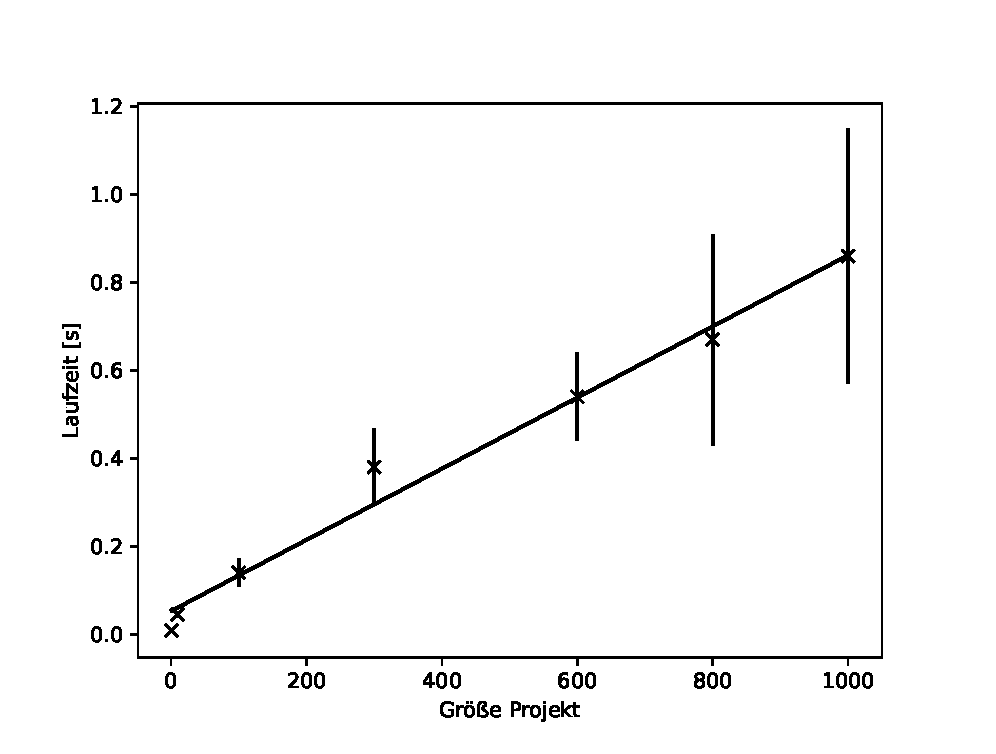
\includegraphics[width=\textwidth]{img/Runtime_Instrumenter.eps}
  \captionof{figure}{Laufzeit des Instrumenters}
  \label{Chap:Tracer-Sec:Laufzeit-Img:LaufzeitInstrumenter}
\end{minipage}
\hfill
\begin{minipage}{0.45\textwidth}
  \centering
  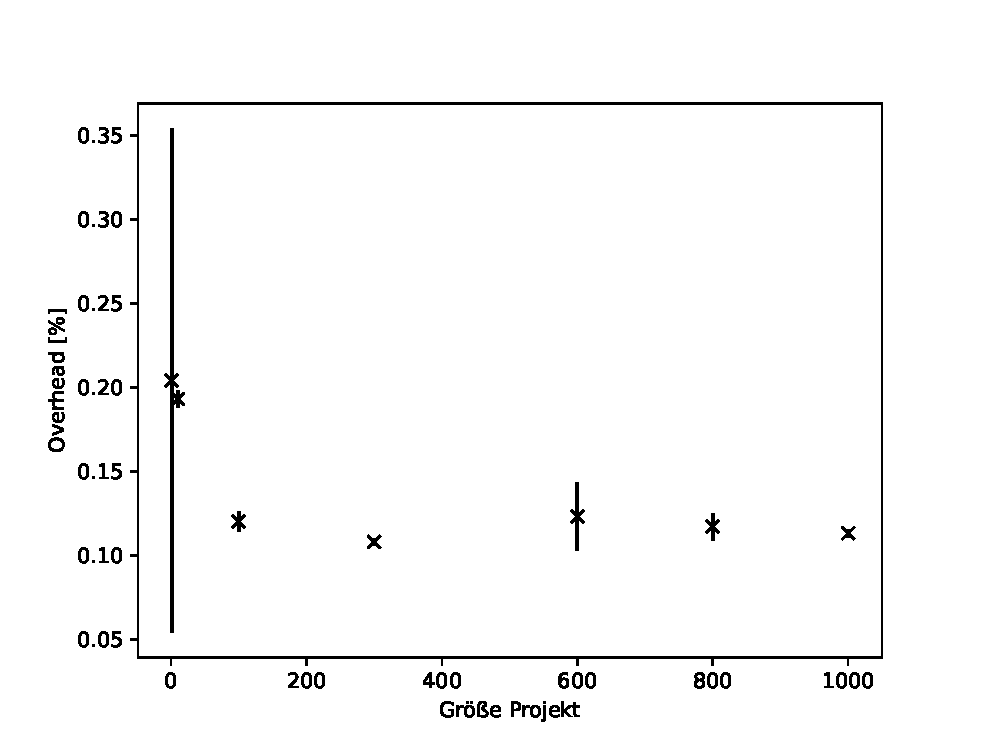
\includegraphics[width=\textwidth]{img/Runtime_Tracer.eps}
  \captionof{figure}{Prozentualer Overhead des Tracers ohne Analyse}
  \label{Chap:Trace-Sec:Laufzeit-Img:LaufzeitTracer}
\end{minipage}
Der abgebildete Graph zeigt die Laufzeit des Programms in $s$ abhängig von der 
Größe des Programms. Das Programm besteht dabei aus einem Testprogramm, welches 
alle möglichen Situationen mit Channels und Mutexen abbildet. Die Vergrößerung 
des Programmes wurde dadurch erreicht, dass die Datei mit dem Programmcode 
mehrfach in dem Projekt vorkam. Ein Projekt mit Größe $n$ besteht vor der 
Instrumentierung also 
aus $n$ Dateien, mit insgesamt $65n$ Zeilen von Code und $52n$ Ersetzungen
in dem AST. Die tatsächliche Laufzeit des Instrumenters auf einen 
Programm hängt schlussendlich natürlich von der tatsächlichen Größe des 
Projekt und der Verteilung der Mutex- und Channel-Operationen in dem Code ab.\\
\begin{table}[!h]
  \centering
  \begin{tabular}{|c|c|c|c|c|}
  \hline
  Projekt & LOC & Nr. Dateien & Nr. Ersetzungen & Zeit {[}s{]} \\ \hline
  ht-cat & $733$ & $7$ & $233$ & $0.013 \pm 0.006$ \\ \hline
  go-dsp & $2229$ & $18$ & $600$ & $0.029 \pm 0.009$ \\ \hline
  goker & $9783$ & $103$ & $4928$ & $0.09 \pm 0.03$ \\ \hline
  \end{tabular}
  \caption{Laufzeit des Instrumenters für ausgewählte Programme}
  \label{Chap:Tracer-Sec:Laufzeit-Tab:LaufzeitInstrumenter}
\end{table}
Zusätzlich wurde die Messung auch mit drei tatsächlichen Programmen 
durchgeführt. Die dort gemessenen Werte befinden sich in 
Tabelle~\ref{Chap:Tracer-Sec:Laufzeit-Tab:LaufzeitInstrumenter}. Gerade in 
Abhängigkeit von der Anzahl der Ersetzungen, stimmen die hier gemessenen Werte
mit denen in Abb.~\ref{Chap:Tracer-Sec:Laufzeit-Img:LaufzeitInstrumenter} gut 
überein, während es bei den anderen Parametern größere Abweichungen gibt.
Dies bestätigt dass der dominante Faktor für die Laufzeit des Programms 
die Anzahl der Ersetzungen in dem AST ist, und die Laufzeit linear von dieser 
abhängt.
\paragraph{Tracer} Folgend soll nun der Overhead des instrumentierten Codes 
im Vergleich zum originalen Code betrachtet werden.
Hierbei wird nur die Laufzeit eines Durchlaufs des eigentlichen Programs
(ohne Wiederholung aufgrund von Select), 
nicht aber der anschließenden 
Analyse betrachtet. Um den Overhead in Abhängigkeit von der Größe des Projektes messen 
zu können, wird das selbe Testprogramm betrachtet, welches bereits in der Messung 
für den Instrumenter verwendet wurde. Abb. \ref{Chap:Trace-Sec:Laufzeit-Img:LaufzeitTracer}
zeigt den gemessenen Overhead. Der durchschnittliche Overhead über alle gemessenen Werte 
liegt dabei bei $14 \pm 2\ \%$. Da der Overhead aber linear davon abhängt, 
wie groß der Anteil der Mutex- und Channel-Operationen im Verhältnis zu 
der Größe bzw. der Laufzeit des gesamten Programms ist, kann dieser Wert abhängig 
von dem tatsächlichen Programm start schwanken. Dies wird unter anderem klar, wenn man 
den Overhead für ht-cat ($9 \pm 3\ \%$) und go-dsp ($60\pm 18\ \%$) welche $51 \pm 21$ 
Prozentpunkte aufeinander liegen. 
